\documentclass[tikz]{standalone}

\usepackage[greek,english]{babel}

\usepackage{pgfplots}
\usetikzlibrary{decorations.pathreplacing}

\pagecolor{white}

\begin{document}
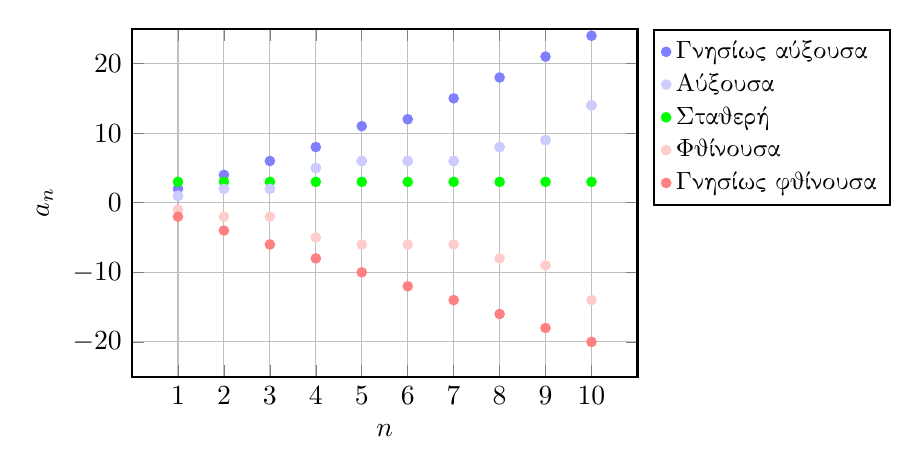
\begin{tikzpicture}
\begin{axis}[
    width=8cm,
    height=6cm,
    domain=-15:15, 
    restrict y to domain=-50:50,
    xmin=0,
    xmax=11,
    ymin=-25,
    ymax=25,
    ytick={-20,-10,0,10,20},
    thick,
    xtick=data,
    legend pos=outer north east,
    mark size=1.5pt,
    xlabel={$n$},
    ylabel={$a_n$},
    legend cell align={left},
    grid]


\addplot[only marks, blue!50!white] coordinates {
(1, 2)
(2, 4)
(3, 6)
(4, 8)
(5, 11)
(6, 12)
(7, 15)
(8, 18)
(9, 21)
(10, 24)
};
\addlegendentry{\small \textgreek{Γνησίως αύξουσα}}

\addplot[only marks, blue!20!white] coordinates {
(1, 1)
(2, 2)
(3, 2)
(4, 5)
(5, 6)
(6, 6)
(7, 6)
(8, 8)
(9, 9)
(10, 14)
};
\addlegendentry{\small \textgreek{Αύξουσα}}

\addplot[only marks, green] coordinates {
(1, 3)
(2, 3)
(3, 3)
(4, 3)
(5, 3)
(6, 3)
(7, 3)
(8, 3)
(9, 3)
(10, 3)
};
\addlegendentry{\small \textgreek{Σταθερή}}

\addplot[only marks, red!20!white] coordinates {
(1, -1)
(2, -2)
(3, -2)
(4, -5)
(5, -6)
(6, -6)
(7, -6)
(8, -8)
(9, -9)
(10, -14)
};
\addlegendentry{\small \textgreek{Φθίνουσα}}

\addplot[only marks, red!50!white] coordinates {
(1, -2)
(2, -4)
(3, -6)
(4, -8)
(5, -10)
(6, -12)
(7, -14)
(8, -16)
(9, -18)
(10, -20)
};
\addlegendentry{\small \textgreek{Γνησίως φθίνουσα}}

\addplot[only marks, blue!20!white] coordinates {
(1, 1)
(2, 2)
(3, 2)
(4, 5)
(5, 6)
(6, 6)
(7, 6)
(8, 8)
(9, 9)
(10, 14)
};


\end{axis}
\end{tikzpicture}
\end{document}
